\chapter{Example Systems with control applications}

\section{Rotor of a Humanoid Robotic arm}

Consider a system of an electric motor given by,
\begin{equation} \label{Eq_2_ch_10_Sys1}
	\ddot{\theta} = \frac{1}{J}(K i - b \dot{\theta})
\end{equation}

there are two highest derivatives in system \eqref{Eq_2_ch_10_Sys1}, considering the both $\ddot{\theta}$ and $\dot{\theta}$ are variables. The control input $u = i$ and the required output of the system is the angular displacement $\theta$. Therefore, the state-space equation can be expressed as,
\begin{align}
	\dot{x} = \begin{bmatrix}
	\dot{\theta} \\ \ddot{\theta}
	\end{bmatrix} &= \begin{bmatrix}
		0 & 1 \\ 0 & -b/J
	\end{bmatrix}\begin{bmatrix}
		\theta \\ \dot{\theta}
	\end{bmatrix} + \begin{bmatrix}
	0 \\ K/J
	\end{bmatrix}u \\
	y &= [1 \quad 0] \begin{bmatrix}
	\theta \\ \dot{\theta}
	\end{bmatrix}
\end{align}

Assume that this system is both completely controllable and observable. For reference tracking, there are two methods, one is the use of reference signal to drive the system to track $r(t)$ by including $-k_{r}r(t)$ for in the control equation itself, as described in section \ref{Example_SingleTrackModel}. Another method is using error dynamics as described here,

for tracking the reference, lets describe error for each of the states as,
\begin{equation}
	\begin{bmatrix}
		\theta - \theta_{d} \\ \dot{\theta}
	\end{bmatrix}
\end{equation}
such that for velocities the reference $\dot{\theta}_{d} = 0$, the reference velocity is when the arm is stabilized to a certain position. 

\section{Full system control design for a single track model}

Consider the already developed single track model linearized as described in \ref{Sec_2_ch_26_SingleTrackModel} also given here,
\begin{equation} \label{Eq_2_ch_27_Model_2_1}
\begin{bmatrix}\dot{v}_y \\ \ddot{\psi} \end{bmatrix} = \begin{bmatrix} -\frac{(c_2 + c_1)}{m v_x} & \frac{-a c_1 + b c_2}{m v_x} - v_x \\
-\frac{a c_1 - b c_2}{J v_x} & \frac{-(a^{2} c_1 + b^{2} c_2)}{J v_x} \end{bmatrix}\begin{bmatrix} v_y \\ \dot{\psi} \end{bmatrix} + \begin{bmatrix} \frac{c_1}{m} \\ \frac{a c_1}{J} \end{bmatrix} \delta
\end{equation}
where $x_1$ is the vehicle's speed, $x_2$ is the yaw-rate and $u$ is the steering angle $\delta$ of the vehicle. Here the state $x_1$ which is $v_y$ and vehicles steering angle $\delta$ ie., $x_2$ are given in the body coordinates. To get the vehicles real position and heading angle in the global reference frame, consider figure \ref{fig_2_ch_27_Model2_1}
\begin{figure}[h!]
	\centering
	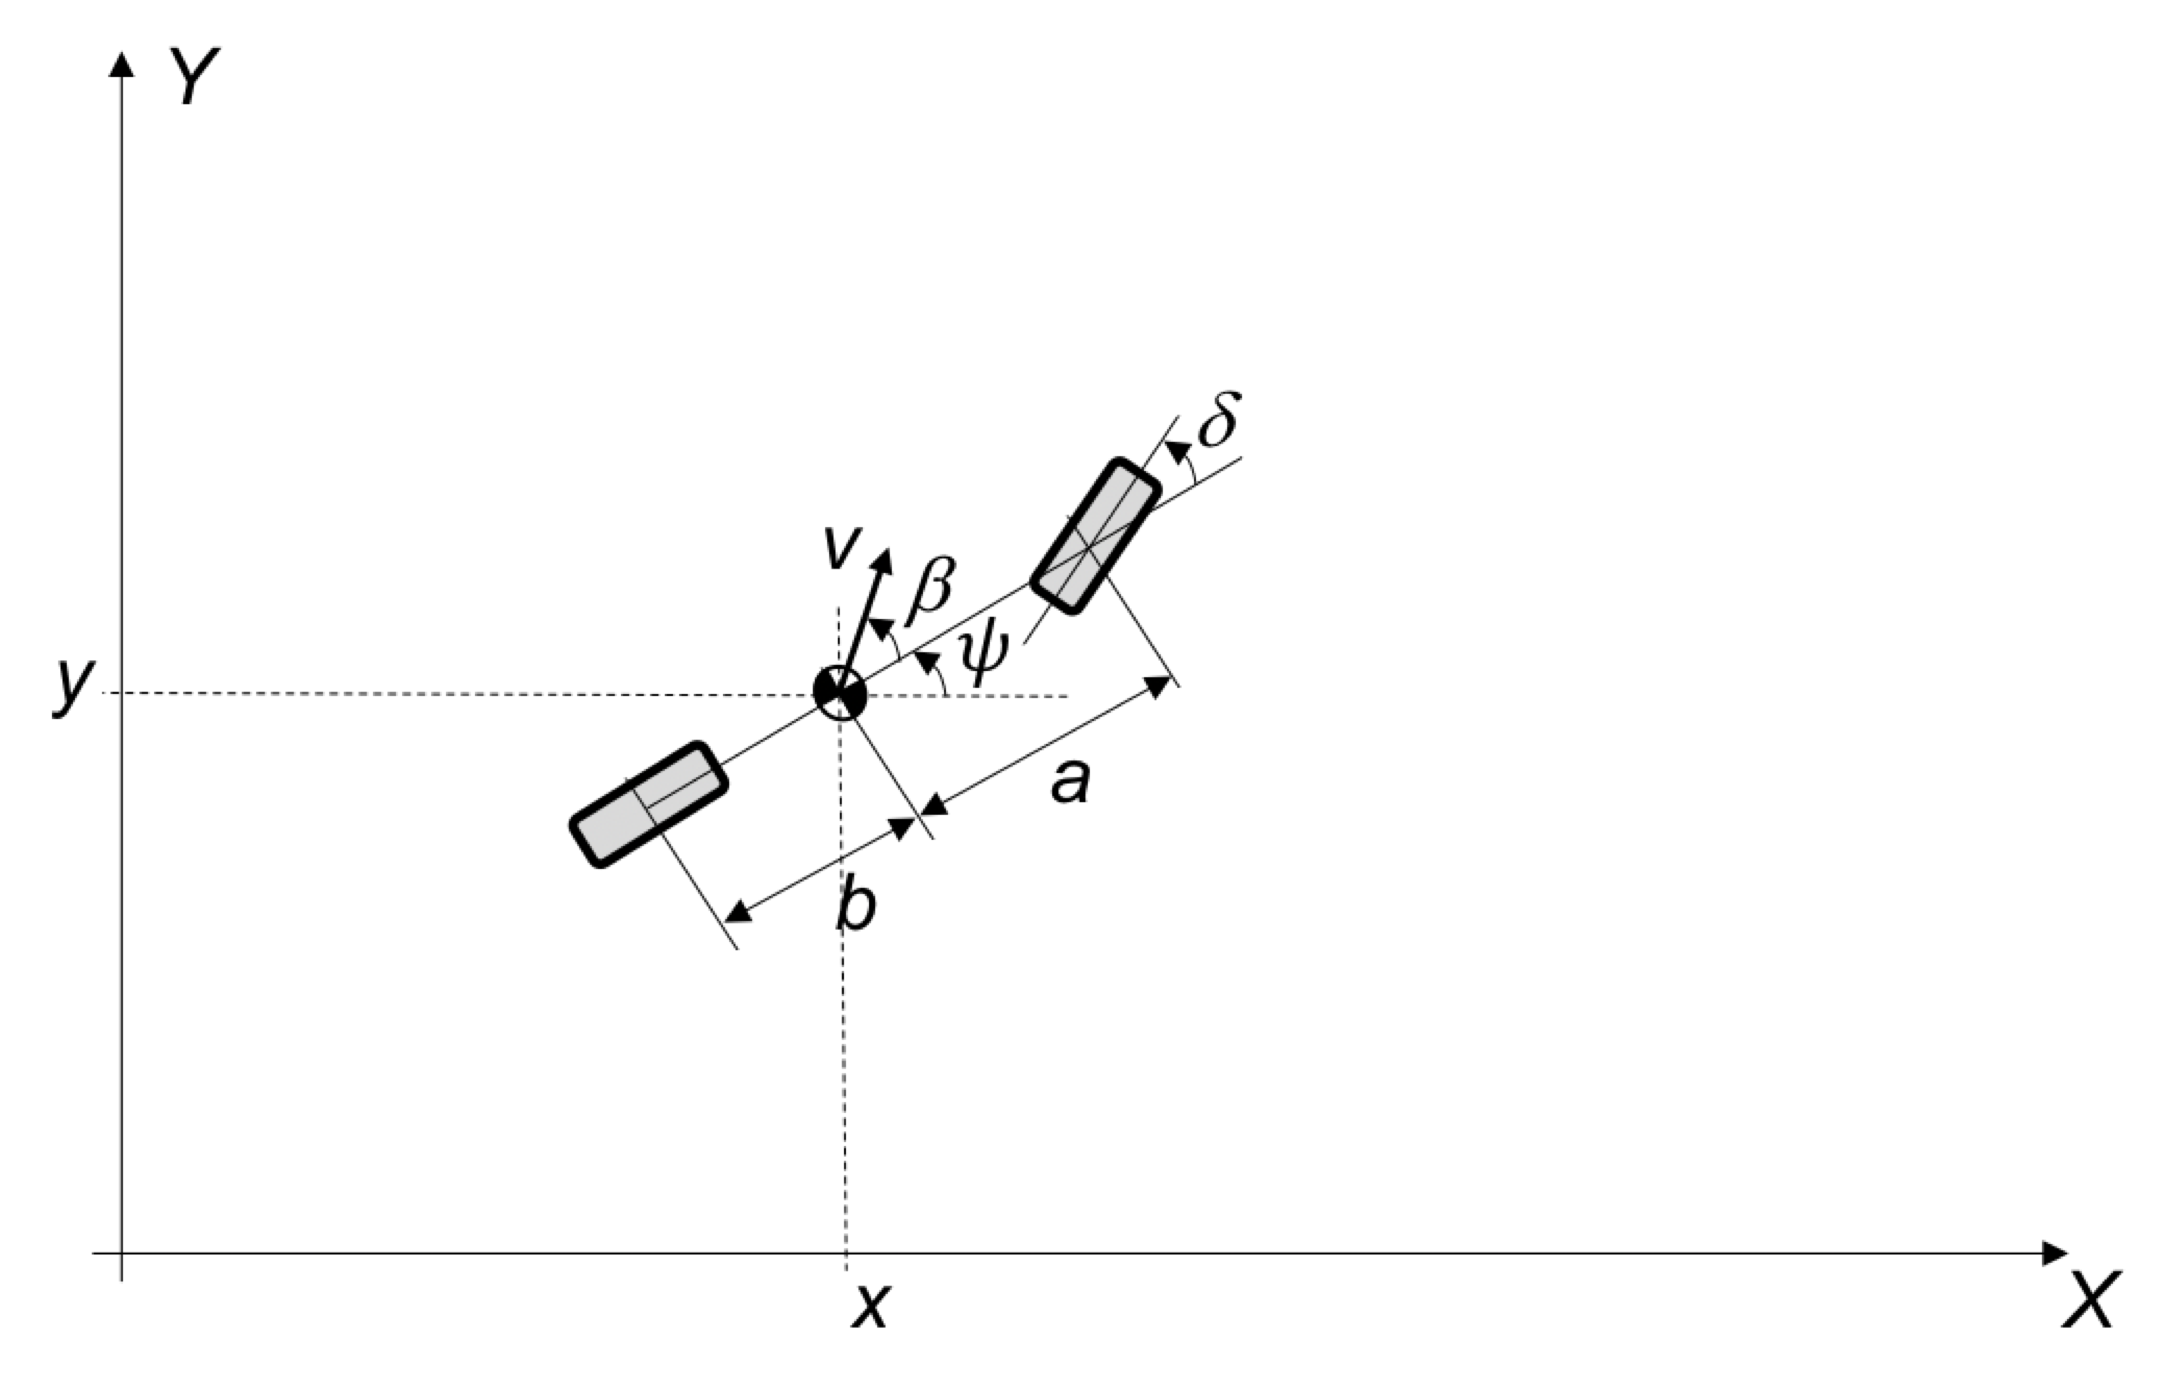
\includegraphics[width=0.7\linewidth]{Bilder/FE_coordinate_system_intro.png}
	\caption{Global coordinate system for single track model}
	\label{fig_2_ch_27_Model2_1}
\end{figure}
using angle cosines, the projections of $v_x$ and $v_y$ on global coordinate system can be determined as,
\begin{align}
	\dot{x} &= v_x cos\psi - v_y sin \psi \\
	\dot{y} &= v_x sin \psi + v_y cos \psi
\end{align}
for this autonomous system, there is an actuator for the steering which is modeled as a non-linear system
\begin{equation}\label{Eq_2_ch_27_Model_2_2}
	\dot{\delta} = -\frac{1}{\tau} \delta + \frac{k_1}{\tau} u + \frac{k_2}{\tau}u^{3}
\end{equation}
where $\delta$ is the steering angle and $u$ is the input voltage to the actuator. Consider the following model parameters given in \ref{Tab_2_ch_27_Model2}
\begin{table}[h!]
	\centering
	\begin{tabular}{p{7cm} p{4cm} p{4cm}}
		\textbf{Description} & \textbf{Parameters} & \textbf{Value}\\
		\toprule[1.5pt]
		vehicle mass & m & 1700 [kg] \\ \cmidrule{1-3}
		vehicle inertia (around z-axis) & J & 2000 [$kg-m^2$] \\ \cmidrule{1-3}
		front wheel cornering stiffness & $c_1$ & 80000 $[kg-m/s^2]$ \\ \cmidrule{1-3}
		rear wheel cornering stiffness & $c_1$ & 100000 $[kg-m/s^2]$ \\ \cmidrule{1-3}
		front wheel to center of mass & a & 1.3 $m$ \\ \cmidrule{1-3}
		rear wheel to center of mass & b & 1.5 $m$ \\ \cmidrule{1-3}
		actuator time constant & $\tau$ & 0.1 $s$ \\ \cmidrule{1-3}
		actuator input gain 1 & $k_1$ & 0.01 $rad/V$ \\ \cmidrule{1-3}
		actuator input gain 2 & $k_2$ & 00056 $rad/V^3$ \\ \bottomrule
	\end{tabular}
	\caption{Single track model parameters}
	\label{Tab_2_ch_27_Model2}
\end{table}

Now with the inclusion of actuator steering dynamics, a new state space model needs to be created. In this single track model, the longitudinal velocity $v_x$ is assumed / maintained constant. Further only lateral dynamics are of concern as a lateral control is developed here. Therefore, the variables that are to be included in order to properly capture all of the lateral dynamics states are as following $[y \quad v_y \quad \psi \quad \dot{\psi}]$ additionally, there is a actuator dynamics variable $\dot{\delta}$ which is also important state to be recorded for a proper lateral control. Therefore, the complete set of states that needs to be considered are as follows
\begin{equation}
	[y \quad v_y \quad \psi \quad \dot{\psi} \quad \delta]^{T} = [x_1 \quad x_2 \quad x_3 \quad x_4 \quad x_5]^{T}
\end{equation}
re-writing the new set of equations for the above mentioned new states in addition to \eqref{Eq_2_ch_27_Model_2_1},
\begin{align}
	\dot{y} &= v_x sin\psi + v_y cos\psi \\
	\dot{v}_y &= -\frac{(c_2 + c_1)}{m v_x} v_y + \left(\frac{-a c_1 + b c_2}{m v_x} -v_x\right)\dot{\psi} + \frac{c_1}{m} \delta \\
	\dot{\psi} &= \dot{\psi} \\
	\ddot{\psi} &= \left(-\frac{a c_1 - b c_2}{J v_x}\right)v_y - \left(\frac{a^2 c_1 + b^2 c_2}{J v_x}\right) \dot{\psi} + \frac{a c_1}{J} \delta \\
	\dot{\delta} &= -\frac{1}{\tau} \delta + \frac{k_1}{\tau} u + \frac{k_2}{\tau}u^{3}
\end{align}
The above set of equations form a set of nonlinear equations describing the dynamics of single track vehicle model concerned only with lateral vehicle dynamics. 

\subsection{Linearizing single track model}
Linearizing the set of nonlinear lateral dynamics single track model as described in the section above such that it can be written in Matrix form $\dot{x} = Ax + Bu$. In order to do so, an operating point has been chosen around $x_e = (0,0,0,0,0)$ and $u_e = 0$. This operating point is chosen such that all lateral motions are zero along with zero inputs for lateral steering, therefore, this operating point $x_e$ denotes a straight forward driving. Using a small step approximation from the operating point of the system as described in chapter Linearization in this book, a set of matrices $A$, $B$ and $C$ are to be developed which denote the Jacobian's of functions with each of the states. These matrices are developed as follows

\begin{equation}
	A = \begin{bmatrix}
	0 & cos\psi & v_x cos\psi - v_y sin\psi & 0 & 0 \\
	0 & -(c_1 + c_2)/m v_x & 0 & -v_x -(a c_1 - b c_2)/m v_x  & c_1 / m \\
	0 & 0 & 0 & 1 & 0 \\
	0 & -(a c_1 - b c_2)/J v_x & 0 & - (c_1 a^2 + c_2 b^2)/J v_x & a c_1 / J \\
	0 & 0 & 0 & 0 & -1/\tau
	\end{bmatrix}_{(x_e, u_e)}
\end{equation}
applying the conditions of operating point,
\begin{equation}
	A = \begin{bmatrix}
	0 & 1 & v_x & 0 & 0 \\
	0 & -(c_1 + c_2)/m v_x & 0 & -v_x -(a c_1 - b c_2)/m v_x & c_1 / m \\
	0 & 0 & 0 & 1 & 0 \\
	0 & -(a c_1 - b c_2)/J v_x & 0 & - (c_1 a^2 + c_2 b^2)/J v_x & a c_1 / J \\
	0 & 0 & 0 & 0 & -1/\tau
	\end{bmatrix}
\end{equation}
similarly, finding the matrix B
\begin{equation}
	B = \begin{bmatrix}
	 0 \\ 0 \\ 0 \\ 0 \\ 3 k_2 u^2 / \tau + k_1 / \tau
	\end{bmatrix}_{(x_e, u_e)} = \begin{bmatrix}
	0 \\ 0 \\ 0 \\ 0 \\ k_1 / \tau
	\end{bmatrix}
\end{equation}
the next step is to design a state feedback controller for the system. Before designing the controller, we need to check if the system is reachable or not.

\subsection{Controllability}
Controllability or more formally reach-ability is the condition from an initial state $x_0$ of a system to reach a controlled state $x_n$ given control input $u$. As described in section of controllabilty in \ref{Sec_2_ch_25_Controllabiliry}, for the case that each of the discrete state ($x_0$ through $x_n$) can be mapped to each of the control inputs ($u_0$ through $u_{n-1}$), the controllabilty matrix $\Gamma$ should be a full row-rank matrix (In linear matrices having a row-rank is same as having a column rank). In other words, having such one-to-one mapping ensures that each of the discrete states are possible by applying required control inputs.

The same of $\Gamma$ depends on the order of the system states, therefore for a five order state system of the linear single track model, the controllabilty matrix is expressed as,
\begin{equation}
	\Gamma = [B \quad AB \quad A^2 B \quad A^3 B \quad A^4 B]
\end{equation}
If $\Gamma$ is a full rank matrix, a test to check weather determinant of $\Gamma \leq 0$ will tell if the rank of $\Gamma$ is not a full rank. In our case, rank($\Gamma$) = $9.5247\times10^5$ which is $\Gamma > 0$, which is a full rank matrix. Therefore, our system with the set of control inputs on steering satisfies that the system is completely controllable. 

\subsection{Feedback Control}

Once the controllabilty is determined, now a controller itself can be designed in order to achieve our target of implementing a lateral control of the vehicle using inputs to the steering. The form of the state-feedback controller should be of,
\begin{equation}
	\Delta u = - K \Delta x + k_r \Delta r
\end{equation}
Before deciding the tuning parameters for the controller, consider the following requirements for the controller.
\begin{itemize}
	\item the lane change maneuver should take not more than 2 seconds
	\item the steady-state vehicle's position should be within the boundary of 5$\%$.
\end{itemize}

The control design is proceeded as follows, the system is of fifth order, therefore, in theory there are five independent poles of the system that can be tuned to bring the system to perform this behavior. For the sake of simplicity, choosing repeated poles such that two repeated poles determine the dynamics of the system. Therefore, being the slowest of the five poles, the other three repeated poles can be placed to be faster than these two first slower repeated poles. Therefore, the required control system should look something like this,
\begin{equation}
	p(s) = (s + p_1)^2 (s + p_2)^3
\end{equation}
the faster poles $p_2$ are chosen at least 3 times faster than $p_1$. Here a simple pole-placement technique is used and Ackermann's formula is used to determine gain $K$ which is detailed in section \ref{Sec_AckermannsFormaula_ControllerTuning} of this book. Now since it is already established that poles $p_2$ should be atleast 3 times bigger than $p_1$, in order to find $p_{des}$ required by Ackermann's formula for controller tuning, there are many possibilities such as the poles being placed at locations as follows $\{p_1, p_2\} = \{ -1,-3 \}$, $\{p_1, p_2\} = \{ -2,-6 \}$, $\{p_1, p_2\} = \{ -3,-9 \}$ or at $\{p_1, p_2\} = \{ -4,-12 \}$. 

Poles $p_1$ being the dominating poles, are selected based on the fact that the setting time as per the requirement should take 2 sec (settling time, here defined as from start of maneuver until the vehicle's position is within $5\%$ of its steady state level). The reference gain should be chosen such that the steady state gain is 1. From the previously listed possibilities of poles $\{p_1, p_2\}$, running simulations can determine the required placement of the poles.







